%%%%%%%%%%%%%%%%%%%%%%%%%%%%%%%%%%%%%%%%%
% Journal Article
% LaTeX Template
% Version 1.4 (15/5/16)
%
% This template has been downloaded from:
% http://www.LaTeXTemplates.com
%
% Original author:
% Frits Wenneker (http://www.howtotex.com) with extensive modifications by
% Vel (vel@LaTeXTemplates.com)
%
% License:
% CC BY-NC-SA 3.0 (http://creativecommons.org/licenses/by-nc-sa/3.0/)
%
%%%%%%%%%%%%%%%%%%%%%%%%%%%%%%%%%%%%%%%%%

%----------------------------------------------------------------------------------------
%	PACKAGES AND OTHER DOCUMENT CONFIGURATIONS
%----------------------------------------------------------------------------------------

\documentclass[10pt]{article} % Single column

%\documentclass[twoside,twocolumn]{article} % Two column

\usepackage{blindtext} % Package to generate dummy text throughout this template 

\usepackage[sc]{mathpazo} % Use the Palatino font
\usepackage[T1]{fontenc} % Use 8-bit encoding that has 256 glyphs
\linespread{1.05} % Line spacing - Palatino needs more space between lines
\usepackage{microtype} % Slightly tweak font spacing for aesthetics

\usepackage[spanish]{babel} % Language hyphenation and typographical rules

\usepackage[hmarginratio=1:1,top=32mm,columnsep=20pt]{geometry} % Document margins
\usepackage[hang, small,labelfont=bf,up,textfont=it,up]{caption} % Custom captions under/above floats in tables or figures
\usepackage{booktabs} % Horizontal rules in tables

\usepackage{lettrine} % The lettrine is the first enlarged letter at the beginning of the text

\usepackage{enumitem} % Customized lists
\setlist[itemize]{noitemsep} % Make itemize lists more compact

\usepackage{abstract} % Allows abstract customization
\renewcommand{\abstractnamefont}{\normalfont\bfseries} % Set the "Abstract" text to bold
\renewcommand{\abstracttextfont}{\normalfont\small\itshape} % Set the abstract itself to small italic text

\usepackage{titlesec} % Allows customization of titles
\renewcommand\thesection{\Roman{section}} % Roman numerals for the sections
\renewcommand\thesubsection{\roman{subsection}} % roman numerals for subsections
\titleformat{\section}[block]{\large\scshape\centering}{\thesection.}{1em}{} % Change the look of the section titles
\titleformat{\subsection}[block]{\large}{\thesubsection.}{1em}{} % Change the look of the section titles

\usepackage{fancyhdr} % Headers and footers
\pagestyle{fancy} % All pages have headers and footers
\fancyhead{} % Blank out the default header
\fancyfoot{} % Blank out the default footer
\fancyhead[C]{Compilaci\'on. \textbf{Cool Compiler 2023}} % Custom header text
\fancyfoot[RO,LE]{\thepage} % Custom footer text

\usepackage{titling} % Customizing the title section

\usepackage{hyperref} % For hyperlinks in the PDF

\usepackage{graphicx} % For images

\usepackage{pifont} % bullets

\usepackage{amsmath}

\usepackage{algpseudocode}

\usepackage{float}
% Keywords command
\providecommand{\keywords}[1]
{
	\small	
	\vspace{0.5em}
	\noindent \textbf{\textit{Palabras clave --- }} #1
}


%----------------------------------------------------------------------------------------
%	TITLE SECTION
%----------------------------------------------------------------------------------------

\setlength{\droptitle}{-4\baselineskip} % Move the title up

\pretitle{\begin{center}\Huge\bfseries} % Article title formatting
	\posttitle{\end{center}} % Article title closing formatting
\title{\normalsize{Compilaci\'on}\\
	\Huge\bfseries Cool Compiler 2023 \\
} % Article title
\author{% 
	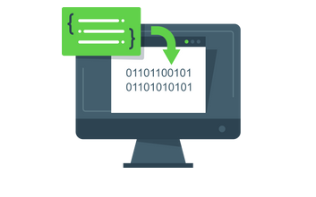
\includegraphics[width=15em]{logo.png}\\
	Karlos Alejandro Alfonso Rodríguez\\
	Laura Victoria Riera P\'erez\\
	Kevin Talavera Díaz \vspace{1em} \\
	\small Cuarto a\~no. Ciencias de la Computaci\'on. \\ % institution
	\small Facultad de Matem\'atica y Computaci\'on, Universidad de La Habana, Cuba \\ % institution
}
\date{\footnotesize \today } % Leave empty to omit a date


% Abstract configurations
\renewenvironment{abstract}
{\small
	\begin{center}
		\bfseries \abstractname\vspace{-.5em}\vspace{0pt}
	\end{center}
	\list{}{
		\setlength{\leftmargin}{1.5cm}%
		\setlength{\rightmargin}{\leftmargin}%
	}%
	\item\relax}
{\endlist}

\usepackage{amsthm}
\usepackage{amssymb}
\usepackage{todonotes} % \TODO
\usepackage{listings} % Code listings
\usepackage{xcolor}

\definecolor{backcolour}{rgb}{0.95,0.95,0.92}

\newcommand{\csl}[1]{\colorbox{backcolour}{\texttt{#1}}}

\newcommand{\imgcaption}[2]{\tiny \textbf{Figura #1.} #2.}

\newcommand{\mgc}[2][]{\colorbox{backcolour}{\texttt{\_\_#2\_\_#1}}}

\newcommand{\mgccapt}[1]{\texttt{\_\_#1\_\_}}

\newtheorem{thm}{Teorema}
\newtheorem{mydef}{Definici\'on}%[section]
\newtheorem{lem}{Lema}
\newtheorem{fig}{\scriptsize{Figura}}


\renewcommand{\qedsymbol}{\rule{0.7em}{0.7em}}

% Hyperlinks configurations
\hypersetup{
	colorlinks=true,
	linkcolor=black,
	filecolor=magenta,      
	urlcolor=cyan,
	pdftitle={Overleaf Example},
	pdfpagemode=FullScreen,
}

%----------------------------------------------------------------------------------------

\begin{document}
	
	\bibliographystyle{ieeetr}
	
	% Print the title
	\maketitle
	
	%----------------------------------------------------------------------------------------
	%	ARTICLE CONTENTS
	%----------------------------------------------------------------------------------------
	
	\section*{Repositorio del proyecto}
	\begin{center}
		\url{https://github.com/computer-science-crows/cool-compiler-2023}
	\end{center}

	\section{Uso del compilador}
	
	Para utilizar el compilador, navegue al directorio /src y ejecute el siguiente comando: \textit{python -m coolcmp -h}, lo que mostrará la ayuda con las opciones disponibles. Para compilar el archivo \textit{code.cl}, simplemente ejecute: \textit{python -m coolcmp code.cl}. Este proceso generará un archivo \textit{code.mips}, que puede ser ejecutado en el simulador SPIM mediante el comando: \textit{spim -f code.mips}.
	
	\begin{figure}
		\centering
		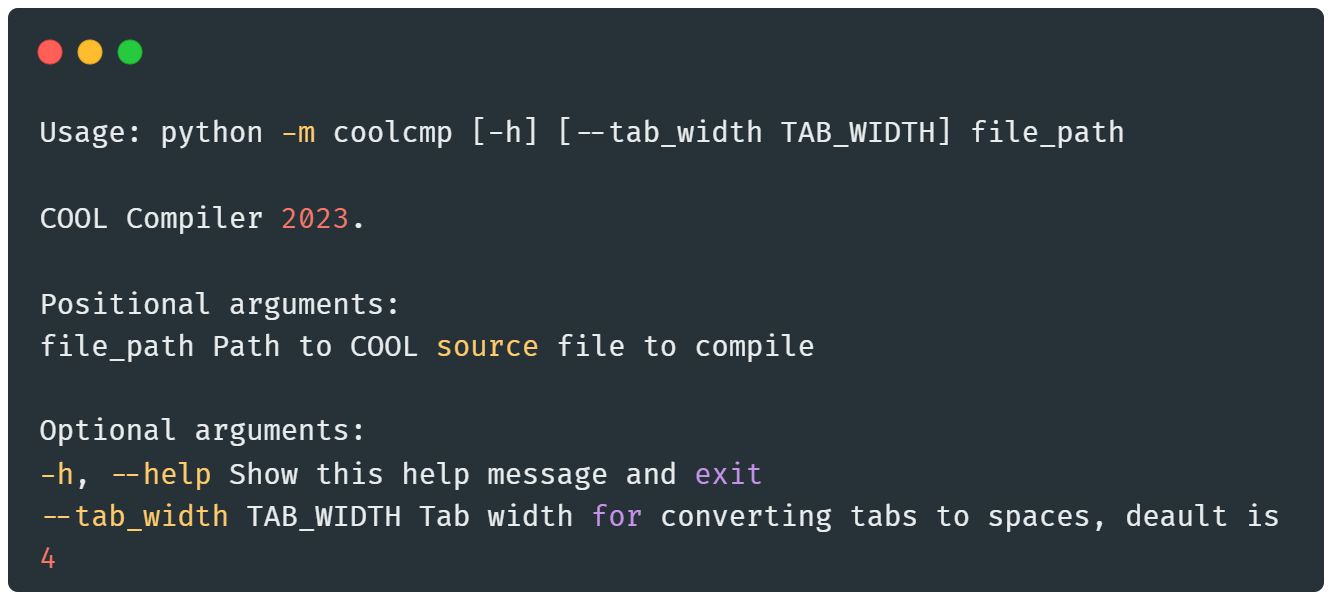
\includegraphics[width=10cm]{usage}
		\caption{Uso del compilador}
	\end{figure}

	\subsection{M\'odulos}
	
	El proyecto está estructurado en varios módulos ubicados en la carpeta /src:
	
	\begin{figure}[H]
		\centering
		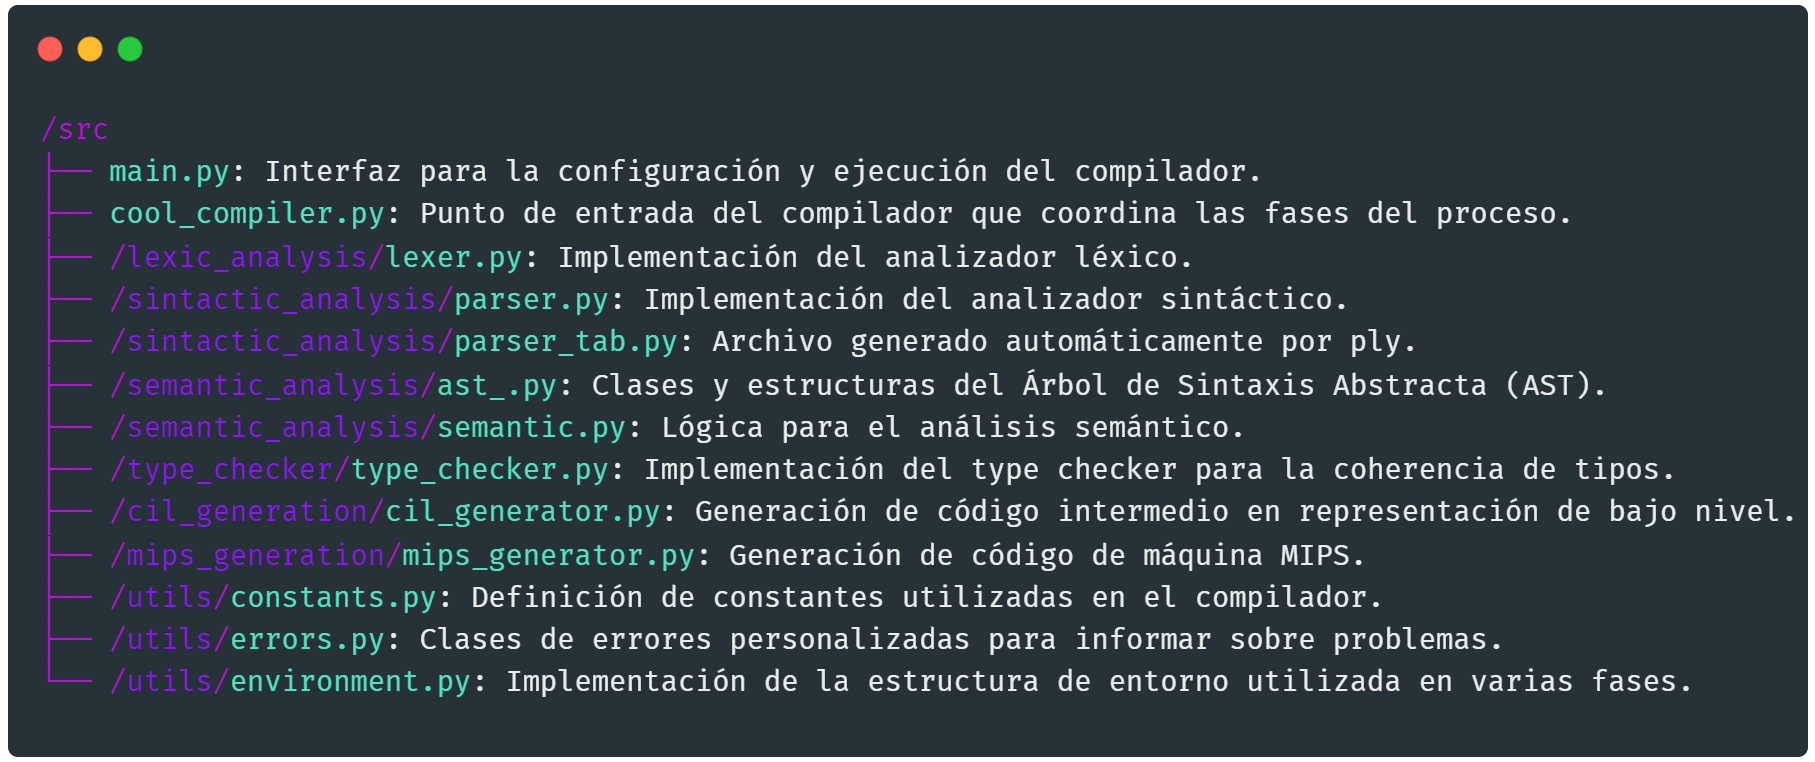
\includegraphics[width=15cm]{structure}
		\caption{Estructura del proyecto}
	\end{figure}

	\subsection{Fases}
	
	El proceso de compilación consta de varias fases esenciales que transforman el código fuente en COOL en un programa ejecutable. Comienza con el análisis léxico, donde se identifican los componentes básicos del código. Luego, el análisis sintáctico verifica la estructura gramatical correcta. A continuación, el análisis semántico evalúa el significado del código. El chequeo de tipos garantiza la coherencia entre los tipos en el programa. La generación de código intermedio crea una representación más abstracta del programa, seguida de la optimización para mejorar el rendimiento. Finalmente, la generación de código de máquinas traduce el programa a instrucciones específicas del hardware para su ejecución. Cada fase desempeña un papel crucial en la creación de un software funcional y eficiente.
	
	\begin{figure}[H]
		\centering
		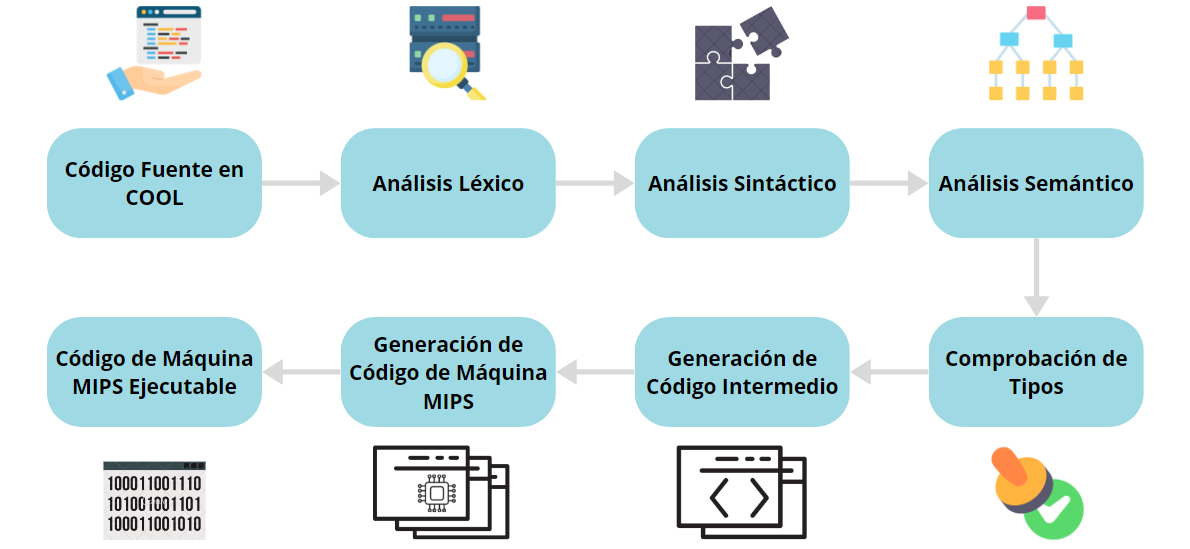
\includegraphics[width=13.5cm]{flow}
		\caption{Flujo del programa}
	\end{figure}
	
	\subsubsection{An\'alisis L\'exico}
	
	\subsubsection{An\'alisis Sint\'actico}
	
	\subsubsection{An\'alisis Sem\'antico}
	
	\subsubsection{Comprobaci\'on de Tipos}
	
	El chequeo de tipos se realiza utilizando el patrón de diseño Visitor, y puede ser encontrado en type\_checker.py.
	
	\vspace{0.5em}
	\begin{itemize}
	\item \textbf{Conformance Test:} Previo al análisis de tipos, es esencial verificar si un nodo U \textit{conforma} con otro nodo V. En este contexto, la conformidad indica que el nodo U puede ser manejado como si perteneciera al tipo del nodo V.
	
	Durante esta validación, se asegura que las expresiones y operaciones del programa sigan las reglas de tipos establecidas por COOL, posibilitando el polimorfismo al permitir que objetos de clases derivadas se utilicen en contextos donde se espera una clase base. La conformidad de tipos se establece en función del árbol de herencia, donde un tipo se considera conforme a otro si comparten el mismo tipo o están en su cadena de herencia. 
	
	Para llevar a cabo esta tarea, se emplea un Depth-First Search (DFS) que calcula dos valores para cada nodo $x$: $td(x)$, el tiempo de descubrimiento de $x$, es decir, el primer momento en que el DFS llega a X; y $tf(x)$, el tiempo de finalización de $x$, es decir, el último momento en que el DFS está en $x$. La relación de conformidad entre dos nodos $U$ y $V$ se verifica mediante las propiedades de $td$ y $tf$. $U$ conforma con $V$ si $td(V) \leq td(U) \leq tf(V)$.
	
	\item \textbf{Lowest Common Ancestor:} La operación \textit{join} en COOL se utiliza para determinar el tipo estático común más bajo de dos tipos dados. Esta operación es necesaria cuando se realiza una operación de "dispatch" o llamada a método en COOL para garantizar que se esté invocando el método correcto según la jerarquía de tipos.
	
	Para encontrar el tipo estático común más bajo, se utiliza el concepto de Lowest Common Ancestor (LCA) o ancestro común más bajo de dos nodos en el AST. La implementación sigue un proceso básico: si el nodo U está más lejos de la raíz que el nodo V, se establece que LCA(U, V) = LCA(padre(U), V). Este proceso se repite hasta que U y V son iguales, momento en el cual el LCA es U. 
	
	\item \textbf{Inicialización del Orden:}
	Durante la traversa DFS del AST, se inicializan los valores td y tf para cada nodo. Además, se verifican las compatibilidades de los métodos heredados y se precálcula el tipo estático de los formales de los métodos antes de la visita.

	\item \textbf{Resolución de Problemas Técnicos:}
	
	Conformidad de Métodos Inherentes: Se asegura que los métodos heredados sean compatibles con los métodos en la clase hija.
	
	Ciclos en la Herencia: Se verifica la presencia de ciclos durante la construcción del árbol de herencia.
	
	Consideraciones
	Ambiente de Tipos: Se mantiene un entorno actual (current\_environment) durante el recorrido del AST para realizar comprobaciones de tipos.
	
	Ámbito de Clases: Se realiza un seguimiento del ambiente de clases actual (current\_class) para lidiar con herencias y definiciones de clases.
	
	\end{itemize}
	
	\subsubsection{Generaci\'on de C\'odigo Intermedio}
	
	\subsubsection{Generaci\'on de C\'odigo de M\'aquina}
	
	\subsection{Gram\'atica}
	
	\section{Problemas técnicos}
	
	\begin{thebibliography}
		a
%		\bibitem{kad} Maymounkov, P., Mazières, D. (2002). \textit{Kademlia: A Peer-to-Peer Information System Based on the XOR Metric.} In: Druschel, P., Kaashoek, F., Rowstron, A. (eds) Peer-to-Peer Systems. IPTPS 2002. Lecture Notes in Computer Science, vol 2429. Springer, Berlin, Heidelberg.
	\end{thebibliography}
\end{document}


